\section{Results}
\frame{\tableofcontents[currentsection, hideothersubsections]}

\begin{frame}
\frametitle{Results: Performance after training}
\begin{figure}
    \centering
    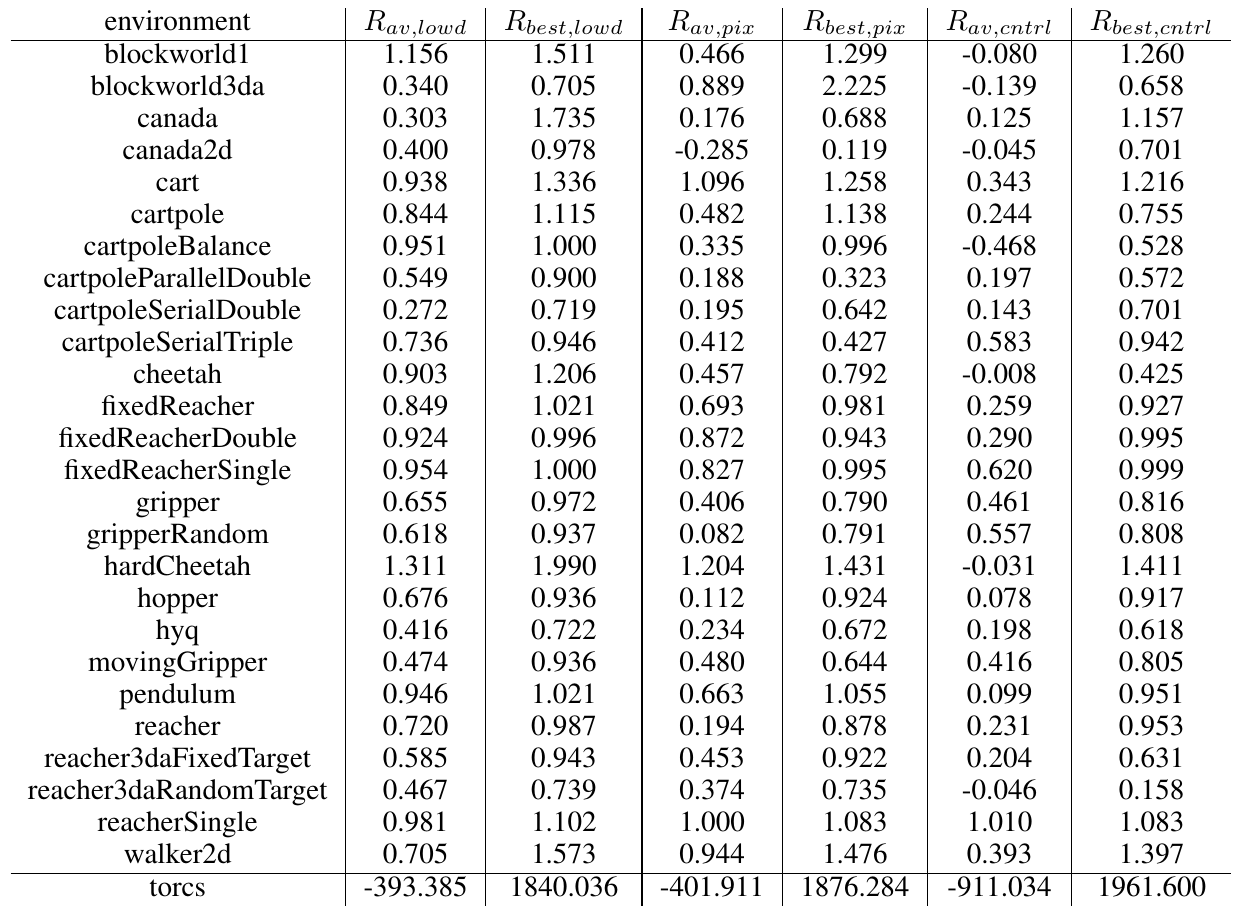
\includegraphics[scale=0.3]{perf_table}
\end{figure}
\end{frame}

\begin{frame}
\frametitle{Results: Estimated Q values}
% \begin{figure}
%     \centering
%     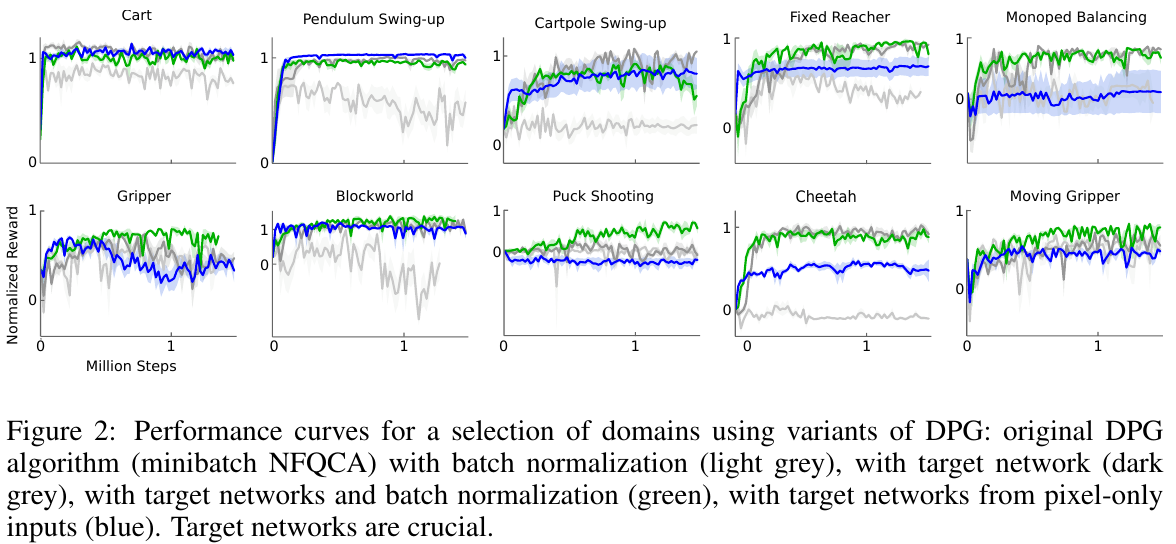
\includegraphics[scale=0.3]{fig_2}
% \end{figure}

\begin{figure}
    \centering
    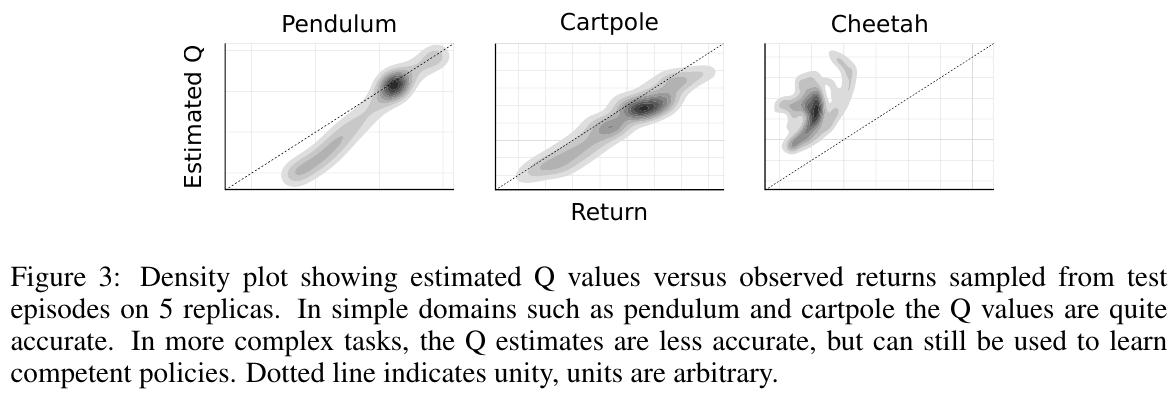
\includegraphics[scale=0.35]{fig_3}
\end{figure}

See: video!
\end{frame}

% \begin{frame}
% \frametitle{Result List}

% \begin{itemize}
%   \item able to find policies whose performance is competitive with those found by a planning algorithm with full access to the dynamics of the domain and its derivatives.
%   \item for many of the tasks the algorithm can learn policies “end-to-end”: directly from raw pixel inputs.
% \end{itemize}

% Surprisingly, in some simpler tasks, learning policies from pixels is just as fast as learning using the low-dimensional state descriptor. This may be due to the action repeats making the problem simpler. It may also be that the convolutional layers provide an easily separable representation of state space, which is straightforward for the higher layers to learn on quickly.

% \end{frame}
